\newpage

\section{Domian Specific Language}

\subsection{Introduction}

A domain-specific language is a computer programming language of restricted expressiveness focused on a particular 
domain\cite{van2000domain}. DSLs are in widespread use in a variety of domains and are becoming more popular. 
Examples of widely used
DSLs are TeX and LaTeX for typesetting academic papers, SQL for database querying, 
Rails for web application development and
VHDL for hardware design. OpenGL can also be viewed as a DSL.
By exposing an interface for specifying polygons and the rules to
shade them, OpenGL created a high-level programming model for
real-time graphics decoupled from the hardware or software used
to render it, allowing for aggressive performance gains as graphics
hardware evolves. The use of DSLs can provide significant gains in
the productivity and creativity of application developers, 
the portability of applications, and application performance.  A programmer using one or
more of these DSLs writes her programs using domain-specific notation and constructs.
 The programs appear sequential and all parallelism and use of the heterogeneous machine resources is implicit.
DSLs raise the level of abstraction and can provide a sequential
model which satisfies the productivity goal.

An additional benefit of using a domain-specific approach is the
ability to use domain knowledge to apply static and dynamic optimizations to a program written using a DSL.
 Most of these domainspecific optimizations would not be possible if the program was
written in a general-purpose language. General-purpose languages
are limited when it comes to optimization for at least two reasons.
First, they must produce correct code across a very wide range of
applications. This makes it difficult to apply aggressive optimizations. 
Compiler developers must err on the side of correctness. 
Second, because of the general-purpose nature needed to support a
wide range of applications (e.g. financial, gaming, image processing, etc.), 
compilers can usually infer little about the structure of
the data or the nature of the algorithms the code is using. DSLs on
the other hand, with their expressive power and knowledge of the
domain’s data structures and algorithms make such optimizations
feasible. This makes DSLs a good choice to deliver on our performance goal. 

Since interesting applications might leverage a variety of DSLs,
it is critical to not only simplify the development of DSLs by 
creating a shared infrastructure, but also to allow these DSLs to interoperate.

The ability to easily embed DSLs simplifies the task of a DSL
developer. However, assistance in parallelizing and targeting heterogeneous resources is also needed. 



\subsection{DSLS FOR HETEROGENEOUS PARALLELISM\cite{brown2011heterogeneous}}

In this section we briefly illustrate the benefits of using
DSLs for achieving both productivity and portable parallel
performance in a heterogeneous environment. We will use
OptiML \cite{sujeeth2011optiml}, a DSL for machine learning, as a running
example. We then address the common challenges faced when
designing and building a new DSL targeted to heterogeneous
parallelism.


\subsubsection{DSL productivity}

At the forefront of DSL design is the ability to exploit
domain knowledge to provide constructs that express domain
operations at a higher level of abstraction. As a consequence of working at this abstraction level much of the lower-level
implementation details are provided by the DSL itself rather
than the application programmer. This often results in a
significant reduction in total number of lines of code as well
as improved code readability compared to a general-purpose
language.

As an example, consider the snippet of OptiML code
shown in Figire \ref{fig:p184}, which shows the core of a downsampling
application. In contrast to the C++ implementation shown in
Figure \ref{fig:p184}, the OptiML version concisely expresses what should
be accomplished rather than how it should be accomplished.

\begin{figure}[H]
	\centering
	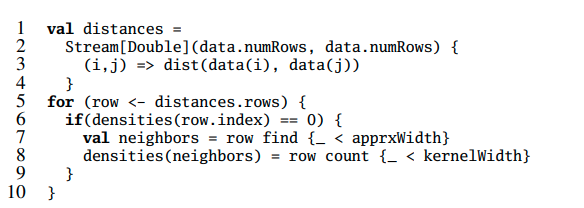
\includegraphics[width=0.6\textwidth]{p187.png}
	\caption{ Downsampling in OptiML}
	\label{fig:p184}
\end{figure}

\begin{figure}[H]
	\centering
	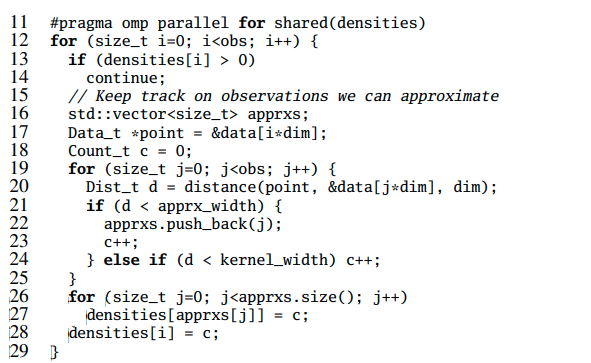
\includegraphics[width=0.6\textwidth]{p188.png}
	\caption{Downsampling in C++}
	\label{fig:p184}
\end{figure}


\subsubsection{Portable parallel performance}
In addition to providing a means of writing concise,
maintainable code, DSLs can also expose significantly more
semantic information about the application than a generalpurpose language. In particular domain constructs can expose
structured, coarse-grained parallelism within an application.
The DSL developer must identify the mapping between domain constructs and known parallel patterns, and with the
proper restrictions this allows the DSL to generate safe and
efficient low-level parallel code from application source using
a sequential programming model.

As an example consider the OptiML sum construct (shown
in \ref{fig:p190}). Summations occur quite frequently in machine
learning applications that focus on condensing large input
datasets into concise, useful output. The construct allows the
user to supply an anonymous function producing the elements
to be summed that is subject to the restricted semantics
enforced by the OptiML compiler. The anonymous function
is not allowed to access arbitrary indices of data structures or
mutate global state. This restriction is not overly constraining
for the majority of use cases and allows the function to
be implemented efficiently as a map-reduce. In addition,
the anonymous function is often non-trivial to evaluate, and
therefore exposes coarse-grained parallelism which can be
exploited to achieve strong scaling.


\begin{figure}[H]
	\centering
	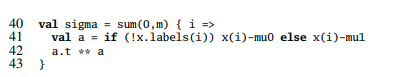
\includegraphics[width=0.6\textwidth]{p190.png}
	\caption{The summation representing the bulk of computation in Gaussian Discriminant Analysis}
	\label{fig:p190}
\end{figure}

Along with the ability to identify the parallelism inherent in an application, domain abstractions can also abstract
away implementation details sufficiently to generate parallel
code optimized for various hardware devices. The lack of
implementation artifacts in the application source ultimately
allows DSL programs to be portable across multiple current
and future architectures.

\subsubsection{Building DSLs}

DSLs have the potential to be a solution for heterogeneous
parallelism, but this solution rests on the challenging task of
building new DSLs targeting parallelism. The first obvious
challenge is designing and constructing a new language,
namely implementing a full compiler (i.e., a lexer, parser, type
checker, analyzer, optimizer, and code generator). In addition,
the DSL must have the facilities to recognize parallelism
in applications, and then to generate parallel code that is
optimized for different hardware devices (e.g., both the CPU
and GPU). This requires the DSL developer to be not only a
domain expert, but also an expert in parallelism (to understand
and implement parallel patterns) as well as architecture (to
optimize for low-level hardware-specific details). Finally, the
DSL developer must write a significant amount of plumbing
whose implementation can have a significant impact on application performance and scalability. This includes choosing
where and how to execute the parallel operations on a given
hardware platform, managing data transfers across address
spaces, and synchronizing reads and writes to shared data.



\subsection{DSL COMPILERS VS. DSL LIBRARIES}

As a simpler alternative to constructing a framework for
building DSL compilers that target heterogeneous hardware,
one could also create a framework for domain-specific libraries. 
In previous work we presented such a framework
along with an earlier version of the OptiML DSL. This
DSL could also target heterogeneous processing elements
transparently from a single application source with no explicit 
parallelism and achieve performance competitive with
MATLAB. These original versions of Delite and OptiML were
implemented as pure libraries in Scala (with the OptiML
library extending the Delite library).






\subsection{Delite}


To address the challenge of building DSLs for parallelism,
 Delite Compiler Framework and Runtime was presented as
a means of dividing the required expertise across multiple
systems developers. Delite uses DSL embedding and an extensible compilation
 framework to greatly reduce the effort
in creating a DSL compiler, provides parallel patterns that
the DSL developer can extend, performs heterogeneous code
generation, and handles all the run-time details of executing
the program correctly and efficiently on various hardware
platforms. In short, Delite provides the expertise in parallelism
and hardware. The DSL developer can then focus on being a
domain expert, designing the language constructs and identifying the mapping 
between those domain constructs and the
parallel patterns Delite provides. He or she must implement the
data and control structures that inherit from Delite prototypes
as well as add domain-specific optimization rules.

The Delite Compiler Framework aims to greatly decrease
the burden of developing a compiler for an implicitly parallel DSL, 
by providing facilities for lifting embedded DSL
programs to an intermediate representation (IR), exposing
and expressing parallelism, performing generic, parallel, and
domain-specific analyses and optimizations, and generating
heterogeneous parallel code that will be executed and managed
by the Delite Runtime.



\subsubsection{Static optimizations and code generation}

By introducing compilation Delite DSLs gain several key
benefits that are crucial to achieving high performance for
certain applications. First of all, we add the ability to perform
static optimizations, which includes generic optimizations provided by the 
Delite framework as well as domain-specific
ones provided by the DSL. With
a library-based approach optimizations can only be performed
dynamically.

In addition, adding code generation support can greatly
improve the efficiency of the final executables by eliminating
all the DSL abstractions and layers of indirection within the
generated code, leaving only type-specialized, straight-line
blocks of instructions and first-order control flow that target
compilers can optimize heavily. Code generating from an IR
also makes targeting hardware other than that supported by
the DSL’s hosting language much more tractable. A common
solution for libraries is to rely on the host language’s compiler to perform code generation for the CPU and manually
provide native binaries targeting other hardware using the host
language’s foreign function interface. In our previous work we
attempted to somewhat ease this burden on the DSL author
for GPUs by writing a compiler plug-in that generated Cuda
equivalents of Scala anonymous functions that had disjoint
data accesses (i.e., maps). By building an IR, however, Delite
is able to handle Cuda code generation seamlessly for both
DSL and user-supplied functions, as well as perform static
optimizations on the generated kernels that are only reasonable
on GPU architectures. These code generators are also easily
extensible to new target languages and architectures, making
the execution target(s) of Delite DSLs truly independent of the
DSL hosting language.


\subsubsection{Runtime optimizations}

It is also important to note that many of Delite’s runtime
features are contingent on full program static analyses, which
are made possible by the compiler statically generating the
execution graph of the application. Delite can make scheduling
decisions and specialize the execution at walk-time, thereby
incurring significantly less run-time overhead. Full program
analysis is also essential for Delite’s ability to manage GPU
memory intelligently, as discussed in Section IV-C. 
A librarybased system can also obtain an execution graph of the
application by dynamically deferring the execution of each
operation and building up the graph at run-time. We employed
such a deferral strategy in our previous work, but were unable
to defer past control flow, thereby creating “windows” of the
application that could be executed at a time. These windows,
however, were not sufficient to allow us to intelligently free
GPU memory. We instead treated the GPU main memory as a
software-managed cache of the CPU main memory, which was
subject to undesirable evictions and could not always handle
application datasets that severely pressured the GPU memory’s
capacity.



\subsubsection{Compilation framework}


The Delite Compiler Framework uses and extends a generalpurpose compiler framework designed for embedding DSLs
in Scala called Lightweight Modular Staging (LMS) \cite{rompf2010lightweight}.
LMS employs a form of meta-programming to construct a
symbolic representation of a DSL program as it is executed.
For DSLs built on top of LMS, the application code is actually
a program generator and each program expression, such as
if (c) a else b, constructs an IR node when the program is
run (in this case \texttt{IfThenElse(c,a,b)}). We use abstract types
and type inference to safely hide the IR construction from the
DSL user \cite{rompf2011building}.

Through this mechanism the DSL compiler effectively
reuses the front-end of the Scala compiler, and then takes
over with the creation of the IR. Possible nodes in the IR
are all constructs of the DSL or constructs the DSL developer
chooses to inherit from Scala (e.g., If-Then-Else statements).
The LMS framework provides all of the tools required for
building the IR, performing analyses and optimizations, and
generating code, which the DSL developer can then use and
extend. Delite expands on this functionality by providing three
primary views of the IR, namely the generic view, the parallel
view, and the domain-specific view, as illustrated in Figure \ref{fig:p189}.


\begin{figure}[H]
	\centering
	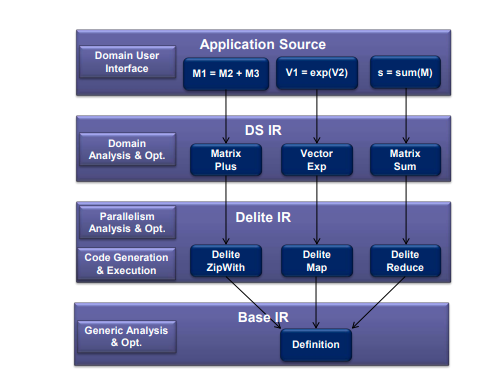
\includegraphics[width=0.6\textwidth]{p189.png}
	\caption{Views of the DSL IR. DSL applications produce an IR
    upon execution. This IR is defined by the LMS framework
    with enough information to perform generic analyses and
    optimizations. The Delite Compiler Framework extends the IR
    to add parallelism information, and this view allows parallel
    optimizations and parallel code generation. The DSL extends
    the parallel IR to form a domain-specific IR, which allows for
    domain-specific optimizations.}
	\label{fig:p189}
\end{figure}

\subsubsection{Gerneric IR}

The lowest-level view of the IR is centered around symbols
and definitions. Unlike many compilers, where individual
statements are fixed to basic blocks, which are connected
in a control flow graph (CFG), we use a "sea of nodes"
representation \cite{paleczny2001java}. Nodes are only connected by their (input
and control) dependencies but otherwise allowed to float freely.
Nodes in the IR are represented as instances of Scala classes;
dependencies are represented as fields in each class. This
representation enables certain optimizations to be performed
during IR construction. For example, when a side-effect free
IR node is constructed, the framework first checks if a definition for the node already exists. If a definition does exist it is
reused to perform global common subexpression elimination
(CSE). Pattern matching optimizations are also applied during
node construction. The DSL compiler can override the construction of an IR node to look for a sequence of operations
and rewrite the entire sequence to a different IR node. This
mechanism is easy to apply and can be used to implement
optimizations such as constant folding and algebraic rewrites.
\ref{fig:p191} shows an example of implementing a simple pattern
matching optimization in OptiML.


\begin{figure}[H]
	\centering
	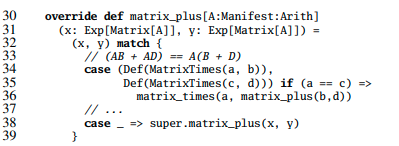
\includegraphics[width=0.6\textwidth]{p191.png}
	\caption{Implementing pattern matching optimizations}
	\label{fig:p191}
\end{figure}

Once the complete IR is built and all dependency information is available, transformations that require a global view
of the program can take place and work towards a program
schedule. Transformations that occur during scheduling include dead-code elimination, various code motion techniques
(e.g., loop hoisting) and aggressive fusing of operations, in
particular loops and traversals. During the course of these
global transformations, the sea of nodes graph is traversed
and the result is an optimized program in block structure.
An important point is that since the IR is composed of
domain operations, all of the optimizations described here are
performed at a coarser granularity (e.g., Matrix-Multiply) than
in a typical compiler.

It is important to note that in a general-purpose environment,
it can be difficult to guarantee the safety of many important optimizations. However, because DSLs naturally use a restricted
programming model and domain knowledge is encoded in
the operations, a DSL compiler can do a much better job at
optimizing than a general-purpose compiler that has to erron the side of completeness. These restrictions are especially
important for tackling side effects in DSL programs in order
to generate correct parallel code.

In the absence of side effects, the only dependencies among
nodes in the IR are input dependencies, which are readily
encoded by references from each node instance to its input
nodes. While Delite and OptiML favor a functional, side-effect
free programming style, prohibiting any kind of side effect
would be overly restrictive and not in line with the driving goal
of offering pragmatic solutions. However, introducing side
effects adds control-, output-, and anti-dependencies that must
be detected by the compiler to determine which optimizations
can be safely performed. Dependency analysis is significantly
complicated if mutable data can be aliased, i.e., a write to one
variable may effect the contents of another variable. The key
to fine-grained dependency information is to prove that two
variables must never alias, which, in general, is hard to do. If
separation cannot be ensured, a dependency must be reported.
Tracking side effects in an overly conservative manner falsely
eliminates both task-level parallelism and other optimization
opportunities.

The approach adopted by Delite is to restrict side-effects to a
more manageable level. Delite caters to a programming model
where the majority of operations is side-effect free and objects
start out as immutable. At any point in the program, however,
a mutable copy of an immutable object can be obtained.
Mutable objects can be modified in-place using side-effecting
operations and turned back into immutable objects, again by
creating a copy. A future version of Delite might even remove
the actual data copies under the hood, based on the results of
liveness analysis. The important aspect is that aliasing (and
deep sharing) between mutable objects is prohibited.

DSL developers explicitly designate effectful operations and
specify which of the inputs are mutated and/or whether the
operation has a global effect (e.g., println). In addition,
developers can specify for each kind of IR node which of
its inputs are only read and which may be aliased by the
object the operation returns (the conservative default being
that any input may be read or aliased). This information is
used by the dependency analysis to serialize reads of anything
that may alias one or more mutable objects with the writes to
those objects. The target of a write, however,  is always known
unambiguously and no aliasing is allowed.


\subsubsection{Parallel IR}

The Delite Compiler extends the generic IR to express
parallelism within and among IR nodes. Task parallelism
is discovered by tracking dependencies among nodes. This
information is used by the Delite Runtime to schedule and
execute the program correctly and efficiently.

IR definition nodes are extended to be a particular kind of
Delite op. There are multiple op archetypes, each of which
expresses a particular parallelism pattern. A Sequential op,
for example, has no internal parallelism, while a Reduce op
specifies the reduction of some collection via an associative operator, and can therefore be executed in parallel (as a treereduce). Delite ops currently expose multiple common dataparallel patterns with differing degrees of restrictiveness. Some
require entirely disjoint accesses (e.g., Map and Zip), while
others allow the DSL to specify the desired synchronization
across shared state for each iteration (e.g., Foreach).

Most Delite data-parallel ops extend a common loop-based
ancestor, the MultiLoop op. A MultiLoop iterates over a
range and applies one or more functions to each index in
the range. MultiLoop also has an optional final reduction
stage of thread-local results to allow Reduce-based patterns to
be expressed. Like Map and Zip, MultiLoop functions must
have disjoint access. However, a MultiLoop may consume
any number of inputs and produce any number of outputs
and is the key abstraction that enables Delite to fuse dataparallel operations together. Delite will fuse together adjacent
or producer-consumer MultiLoops that iterate over the same
range and do not have cyclic dependencies, creating a single
pipelined MultiLoop. By fusing a MultiLoop that produces
a set of elements together with a MultiLoop that consumes
the same set, potentially large intermediate data structures
can be entirely eliminated. Since fusing ops can create new
opportunities for further optimization, fusion is iterated (and
previously discussed optimizations reapplied) until a fixed
point is reached. In addition to allowing multiple data-parallel
ops in a single loop, fusion also effectively creates optimized
MapReduce and ZipReduce ops (as well as any other combination, e.g., MapReduceReduce). Since Delite ops internally
extend MultiLoop, DSL authors can benefit from fusion even
while using only the simpler data parallel patterns.

Fusion can significantly improve the performance of applications by improving cache behavior and reducing the total
number of memory accesses required. For example consider
the OptiML code shown in \ref{fig:p184}. The application performs
multiple subsequent operations on the input in order to update
the result. Fusing these operations into a single traversal over
the input collection that generates all of the outputs at once
without temporary buffer allocations can produce a significant
performance improvement for large inputs.

\subsubsection{Domain-specific IR}

The DSL developer extends the Delite Compiler to create
domain-specific IR nodes that extend the appropriate Delite
op. It is through this simple mechanism that a DSL developer expresses how to map domain constructs onto existing parallel patterns. This highest-level view of the IR is
unique for each DSL and allows for domain-specific analyses
and optimizations. For example, OptiML views certain IR
nodes as linear algebra operations, which allows it to use
pattern matching to apply linear algebra simplification rules.
These rewrites can eliminate redundant work (e.g., whenever
Transpose(Transpose(x)) is encountered, it is rewritten to be
simply x) as well as yield significantly more efficient implementations that are functionally equivalent to the original. As
an example, consider the snippet of OptiML code for Gaussian
Discriminant Analysis (GDA) shown in \ref{fig:p190}. The OptiML compiler’s pattern matcher recognizes that a summation of
outer products can be implemented much more efficiently as
a single matrix multiplication \cite{sujeeth2011optiml}. Specifically, it recognizes


$$
\sum_{i=0}^n \vec{x}_i * \vec{y}_i \rightarrow \sum_{i=0}^n X(:, i) * Y(i,:)=X * Y
$$

The transformed code allocates two matrices, populates
them by performing the operations required to produce all
of the inputs to the original outer product operation, and then
performs the multiplication.



\subsubsection{Heterogeneous code generation}
The final stage of compilation is code generation. The
DSL can extend one or more code generators, which are
modular objects that translate IR nodes to an implementation
in a lower level language. The LMS framework provides the
basic mechanisms for traversing the IR and invoking the code
generation method on each node. It also provides generator
implementations for host language operations. On top of that,
the Delite Compiler Framework supplies generator implementations for all Delite ops. Due to the ops’ deterministic access
patterns and restricted semantics, Delite is able to generate
safe parallel code for CMPs and GPUs without performing
complex dependency analyses. The DSL developer can also
choose to override the code generation for an individual target
(e.g., Cuda \cite{CUDAZone76:online}) to provide a hand-optimized implementation
or utilize an existing library (e.g. CUBLAS, CUFFT). We
currently have implemented code generators for Scala, C++,
and Cuda, which allow us to leverage their existing compilers
to perform further low-level optimizations.

The Delite Compiler Framework adds a new code generator
which generates a representation of the application as an execution graph of Delite ops with executable kernels. The design
supports control flow nodes and nested graphs, exposing parallelism within a given loop or branch. For every Delite op, the
Delite generator emits an entry in the graph containing the op’s
dependencies. It then invokes the other available generators
(Scala, Cuda, etc.) for each op, generating multiple devicespecific implementations of each op kernel. For example, if
a particular operation may be well-suited to GPU execution,
the framework will emit both a CPU-executable variant of
the op as well as a GPU-executable variant of the op. The
runtime is then able to select which variant to actually execute.
Since it is not always possible to emit a given kernel for
all targets, each op in the graph is only required to have at
least one kernel variant. By emitting this machine-agnostic
execution graph of the application along with multiple kernel
variants, we are able to defer hardware specific decisions to
the runtime and therefore run the application efficiently on a
variety of different machines. This mechanism also allows the
DSL to transparently expand its set of supported architectures
as new hardware becomes available. Once Delite supports code
generation and runtime facilities for the new hardware, existing
DSL application code can automatically leverage this support
by simply recompiling.


\subsection{HETEROGENEOUS RUNTIME}

The Delite Runtime provides services required by DSLs to
execute implicitly parallel programs, such as scheduling, data
management, and synchronization, and optimizes execution for
the particular machine.


\subsubsection{Scheduling}

The runtime takes as input the execution graph generated by
the Delite Compiler, along with the kernels and any additional
necessary code generated by the Delite Compiler, such as DSL
data structures. The execution graph is a machine-agnostic
description of the inherent parallelism within the application that enumerates all the ops in the program along with
their static dependencies and supported target(s). The runtime
schedules the application at walk-time \cite{fisher1997walk}, combining the
static knowledge of the application behavior provided by the
execution graph with a description of the current machine,
i.e., the number of CPU cores, number of GPUs, etc. (see
Figure \ref{fig:p192}). The scheduler traverses all of the nested graphs
in the execution graph file and produces partial schedules for
blocks of the application that are statically determinable. The
partial schedules are dispatched dynamically during execution
as the branch directions are resolved. The runtime scheduler
currently utilizes a clustering algorithm that prefers scheduling
each op on the same resource as one of its inputs. If an
op has no dependencies it is scheduled on the next available
resource. This algorithm attempts to minimize communication
among ops and makes device decisions based on kernel and
hardware availability. Data-parallel ops selected for CMP
execution are split into a number of chunks (determined by
resource availability) and then scheduled across multiple CPU
resources.


\begin{figure}[H]
	\centering
	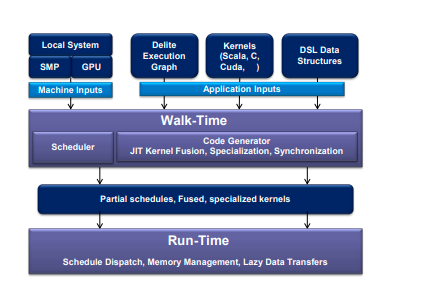
\includegraphics[width=0.6\textwidth]{p192.png}
	\caption{An overview of the Delite Runtime. The runtime
    uses the machine-agnostic execution graph representing the
    application as well as a machine description to schedule and
    execute the application on the available hardware. Walk-time
    code generation utilizes scheduling information to optimize
    kernels and synchronization, minimizing run-time overheads.
    Run-time systems execute the schedule, manage memory, and
    perform data transfers.}
	\label{fig:p192}
\end{figure}

\subsubsection{Schedule compilation}


In order to avoid the overheads associated with dynamically interpreting the execution graph, the runtime generates
an executable for each hardware resource that invokes the
kernels assigned to that resource according to the partial
schedules. Since the compiler is machine-agnostic, the runtime
is responsible for generating an implementation of each dataparallel op that is specialized to the number of processors
chosen by the schedule. For example, a Reduce op only has its
reduction function generated by the compiler, and the runtime
generates a tree-reduction implementation with the tree height
specialized to the number of processors chosen to perform the
reduction.

The generated code enforces the schedule by synchronizing
kernel inputs and outputs across resources. The synchronization is implemented 
by transferring data through lock-based one-place buffers. This code generation allows for a distributed
program at runtime (no master coordination thread is required)
and also allows for multiple optimizations that minimize runtime overhead. For example, kernels scheduled on the same
hardware resource with no communication between them are
fused to execute back-to-back. All synchronization in the
application is generated at this time and only when necessary
(kernel outputs that do not escape a single hardware resource
require no synchronization). So in the simplest case of targeting a traditional uniprocessor, the final executable code will
not invoke any synchronization primitives (e.g., locks). The
runtime also injects data transfers when the communicating
resources reside in separate address spaces. When shared
memory is available, it simply passes the necessary pointers.


\subsubsection{Execution}

The current implementation of the Delite Runtime is written
in Scala and generates Scala code for each CPU thread and
Cuda code to host each GPU. This environment allows it to
support the execution of Scala kernels, C++ kernels, and Cuda
kernels that are generated by the Delite compiler (using JNI
as a bridge). The runtime spawns a JVM thread for each CPU
resource assigned to a kernel, and also spawns a single CPU
host thread per Cuda-compliant GPU.

The GPU host thread performs the work of launching
kernels on the GPU device and transferring data between
main memory and the device memory. For efficiency, it allows
the address spaces to become out-of-sync by default, and
only performs data transfers when the schedule requires them.
Delite also provides memory management for the GPU. Before
each Cuda kernel is launched, any memory on the device it
will require is allocated and registered. The runtime uses the
execution graph and schedule to perform liveness analysis for
each input and output of GPU ops to determine the earliest
time during execution at which it can be freed. By default,
the runtime attempts to keep the host thread running ahead
as much as possible by performing asynchronous memory
transfers and kernel launches. When this causes memory
pressure, however, the runtime uses the results of the liveness
analysis to wait for enough data to become dead, free it, and
then perform the new allocations. This analysis can be very
useful due to the limited memory available in current GPU
devices.